\begin{problem}
How many ways can 7 people stand in a line?
\end{problem}

\begin{problem}
I want to order a cake. There are three layers I can put on the cake, and I can choose from 5 different colors. If I cannot repeat any colors, what is the total number of cakes I can make?
\end{problem}

\begin{problem}
A regular icosahedron is a $20$-faced solid where each face is an equilateral triangle and five triangles meet at every vertex. The regular icosahedron shown below has one vertex at the top, one vertex at the bottom, an upper pentagon of five vertices all adjacent to the top vertex and all in the same horizontal plane, and a lower pentagon of five vertices all adjacent to the bottom vertex and all in another horizontal plane. Find the number of paths from the top vertex to the bottom vertex such that each part of a path goes downward or horizontally along an edge of the icosahedron, and no vertex is repeated. (\textit{Source: AIME I \#3 2016})
 \begin{center}
 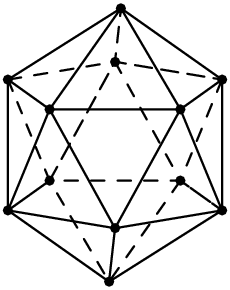
\includegraphics[width=2in]{iso}
 \end{center}
\end{problem}

\begin{problem}
Of the 15 players on a soccer team, 13 are starters. How many different teams of 13 starters are possible?
\end{problem}

\begin{problem}
How many ways can I arrange the word ``MATHCOUNTS''?
\end{problem}

\begin{problem}
How many ways can I arrange the word ``MISSISSIPPI''?
\end{problem}

\begin{problem}
How many ways can I arrange the word ``VIRGINIA'' if the V always has to be next to the A? (e.g. ``VAIRGINI'' or ``GINAVIRI'' both work)
\end{problem}

\begin{problem}
If I want to put 7 balls in a row, 2 that are red, 3 that are blue, and 2 that are green (same colors are indistinguishable), how many ways can I do so?
\end{problem}

\begin{problem}
 How many ways are there to get from the lower left hand corner to the upper right hand corner of the grid below by only using moves that are right or up?
 \begin{center}
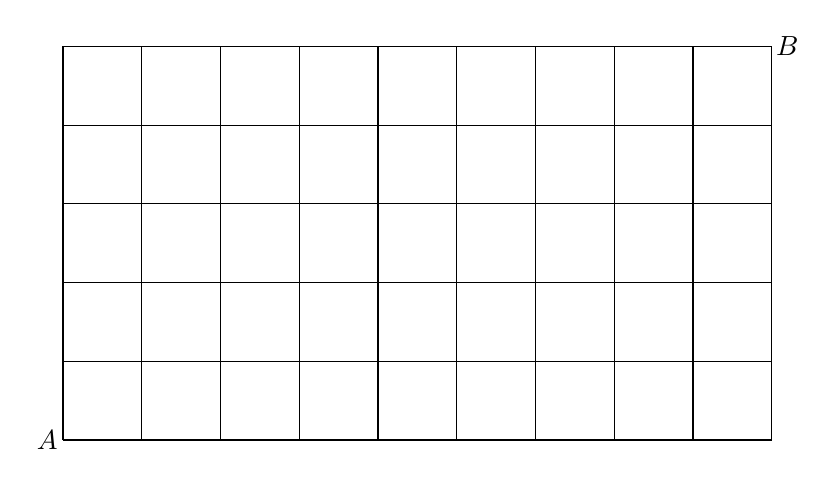
\begin{tikzpicture}
		\draw (0,0) grid (9,5);
		\node (a) at (-0.2, 0) {$A$}; 
		\node (b) at (9.2, 5) {$B$}; 
\end{tikzpicture}
\end{center}
\end{problem}

\begin{problem}
 I am currently at home ($A$) and I want to make my way to work at $B$. However, I know there is an accident at point $C$ and $D$ in the city, so I want to avoid routes that pass through those places. Taking this into consideration, how many ways can I drive from $A$ to $B$ if I must not pass through $C$ \textit{or} $D$?
 \begin{center}
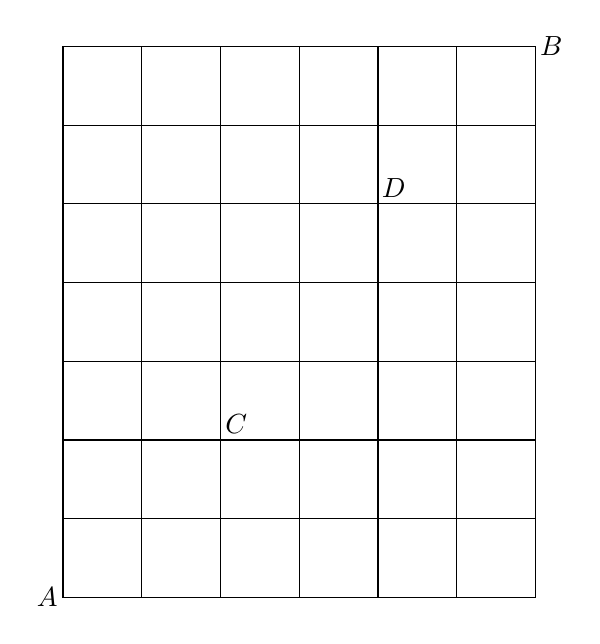
\begin{tikzpicture}
		\draw (0,0) grid (6,7);
		\node (a) at (-0.2, 0) {$A$}; 
		\node (c) at (2.2, 2.2) {$C$};
		\node (d) at (4.2, 5.2) {$D$};
		\node (b) at (6.2, 7) {$B$}; 
\end{tikzpicture}
\end{center}
 \end{problem}

\begin{problem}
I am walking a 3-D grid. If I want to get from (0,0,0) to (2,5,4), how many paths are possible?
\end{problem}

\begin{problem}
$^{\ast \ast \ast}$ Dizzy Daisy is standing on the point (0, 0) on the $xy$-plane and is trying to get to the point (6, 6). She starts facing rightward and takes a step 1 unit forward. On each subsequent second, she either takes a step 1 unit forward or turns 90 degrees counterclockwise then takes a step 1 unit forward. She may never go on a point outside the square defined by $\abs{x} \leq 6, \,\, \abs{y} \leq 6$, nor may she ever go on the same point twice. How many different paths may Daisy take? (\textit{Source: HMMT})
\end{problem}